\documentclass[a4paper]{article}

\usepackage[utf8x]{inputenc}

\usepackage[left=2cm,top=2cm,right=2cm,bottom=2cm]{geometry}

\usepackage{geometry}
\geometry{a4paper}

\usepackage{graphicx}

\usepackage{minted}
% global minted style  
\setminted{  
encoding=utf-8
}

\usepackage{fancyhdr}

\pagestyle{fancy}
\fancyhf{}
\rhead{Palvinder Sander}
\lhead{Machine Learning Assessment One}
\rfoot{Page \thepage}

\usepackage{mathpartir}

\usepackage{bussproofs}
\usepackage{cancel}
\usepackage{tabularx}

\usepackage{amsmath,bm}
\usepackage{unicode-math}
\setmathfont[]{CambriaMath}
\setmathfont[version=bold,FakeBold=2]{CambriaMath}

%\usepackage{tcolorbox}
%\usepackage{etoolbox}
%\BeforeBeginEnvironment{minted}{\begin{tcolorbox}}%
%\AfterEndEnvironment{minted}{\end{tcolorbox}}%

\title{Logic Assessment One}
\author{Palvinder Sander}
\date{}

\begin{document}

\section*{Question One:}

%\inputminted[frame=single,framesep=10pt,mathescape=true,escapeinside=||]{java}{nonLinearReg.java}

Univariate non-linear regression in Java with inital values of $w_{0}$, $w_{1}$ and $w_{2}$ set to $0$ and $\alpha$ set to $0.00000001$ over $10000$ epochs. My code\footnote{solution1.java} yields the following hypothesis function and the associated weights:

\begin{minted}[frame=single,framesep=10pt,mathescape=true,escapeinside=||]{java}
>> h(x) = (1.0002793258507536 * x^2) + (0.9820597257019426 * x) + 0.0011254551807739726
>> w2 = 1.0002793258507536
>> w1 = 0.9820597257019426
>> w0 = 0.0011254551807739726
\end{minted}

\noindent After plotting this function (using xchart) we can see parameterized hypothesis function fits the training data very well.

\begin{figure}[h]
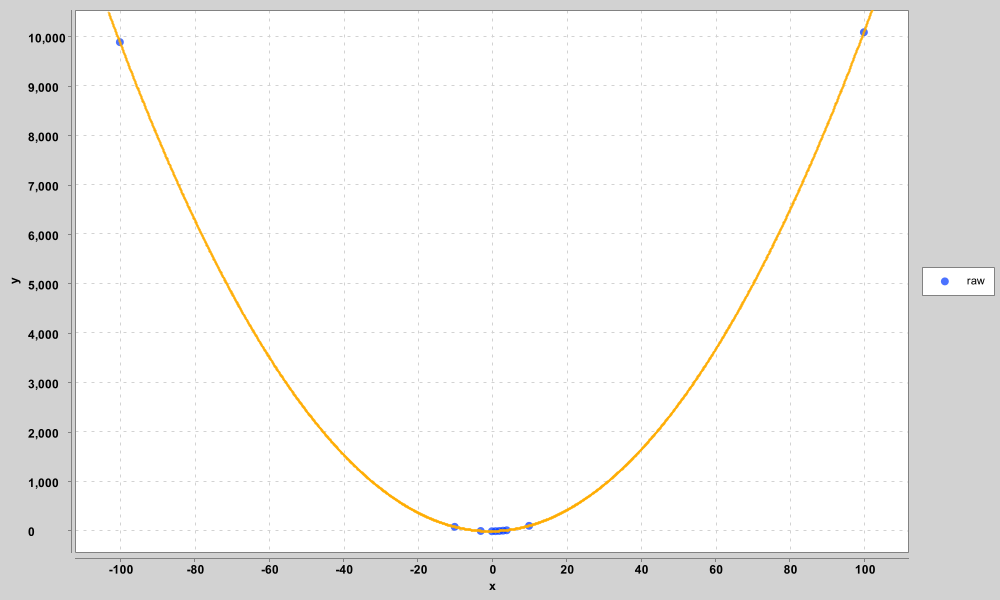
\includegraphics[scale=.4]{g1.png}
\centering
\end{figure}

\noindent My code also outputs how much the cost changes by each time it is incremented; I have shown the last few lines below:

\begin{minted}[frame=single,framesep=10pt,mathescape=true,escapeinside=||]{java}
>> ...
>> 0.8944456993148866
>> 0.9977505546102384
>> 1.0340802667750915
>> 1.0713852057181472
>> 1.1096817412523137
>> 1.1489847692011224
>> 1.4069516500592667
>> 12.709029785778215
\end{minted}

\noindent As you can see, the cost is is normally $\approx 1$; however at the end it peaks to $\approx 12$. The cost is the squared difference between the actual and predicted y co-ordinate of a point. This cost is the last one output and thus is in relation to the point $(100,10101)$. Since this point is so far away from the rest of the data (that it could even be statistically classed as an outlier) the deviation of the hypothesis function is expected to be incorrect by this amount ($\sqrt{12}$).\newpage

\section*{Question Two:}
Multivariate Logistic Regression with inital values of $w_{0}$, $w_{1}$ and $w_{2}$ set to $0$ and $\alpha$ set to $0.1$ over $100$ epochs. My code\footnote{solution2.java} yields the following hypothesis function and the associated weights:
\begin{minted}[frame=single,framesep=10pt,mathescape=true,escapeinside=||]{java}
>> h(x) = (((-2.634179597653396) * x) - -6.816144929215793) / -6.816144929215793
>> w2 = -6.816144929215793
>> w1 = 2.634179597653396
>> w0 = -6.816144929215793
\end{minted}

\noindent After plotting this function (using xchart) we can see the decision boundary function fits the separate classes of points quite well.

\begin{figure}[h]
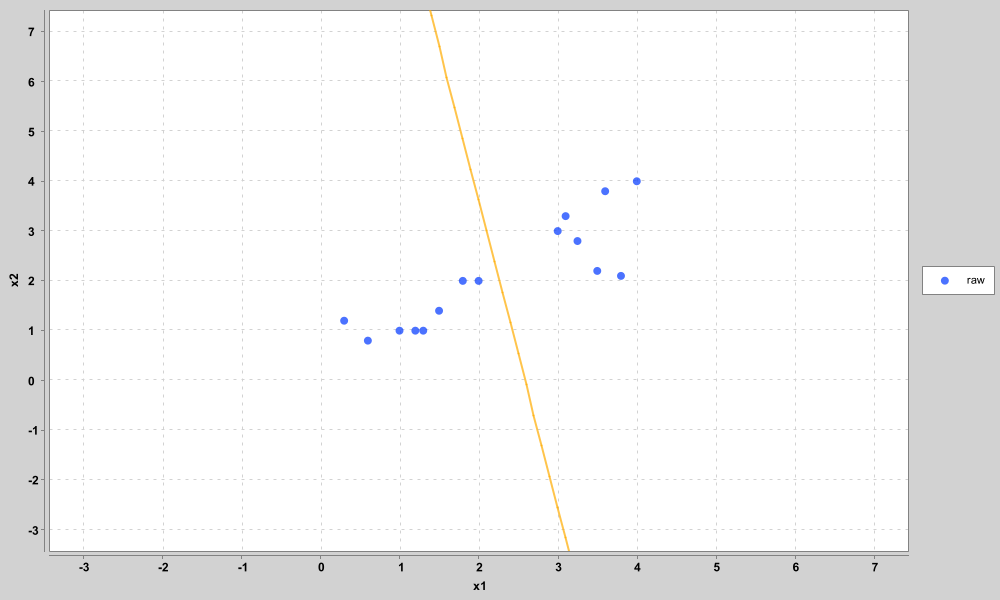
\includegraphics[scale=.4]{g2.png}
\centering
\end{figure}

\noindent My code also outputs how much the cost changes by each time it is incremented; I have shown the last few lines below:

\begin{minted}[frame=single,framesep=10pt,mathescape=true,escapeinside=||]{java}
>> ...
>> -4.199751525602771
>> -2.7425767118276188
>> -3.706825493597943
>> 0.1884845652501731
>> 0.008095068678063375
>> 0.09704676876513688
>> 0.018663634040316904
>> 0.020720688977319088
>> 0.04128209235201255
>> 0.05719333010465827
\end{minted}

\noindent As you can see the cost is strictly decreasing after each iteration. This means that my decision boundry function is converging to an accurate result.

\newpage

\section*{Question 3:}

Neural Network capable of performing the XNAND\footnote{$(x_1 \wedge \neg x_2) \vee (\neg x_1 \wedge x_2)$} operation on two variables $x_1$ and $x_2$:
\begin{figure}[h]
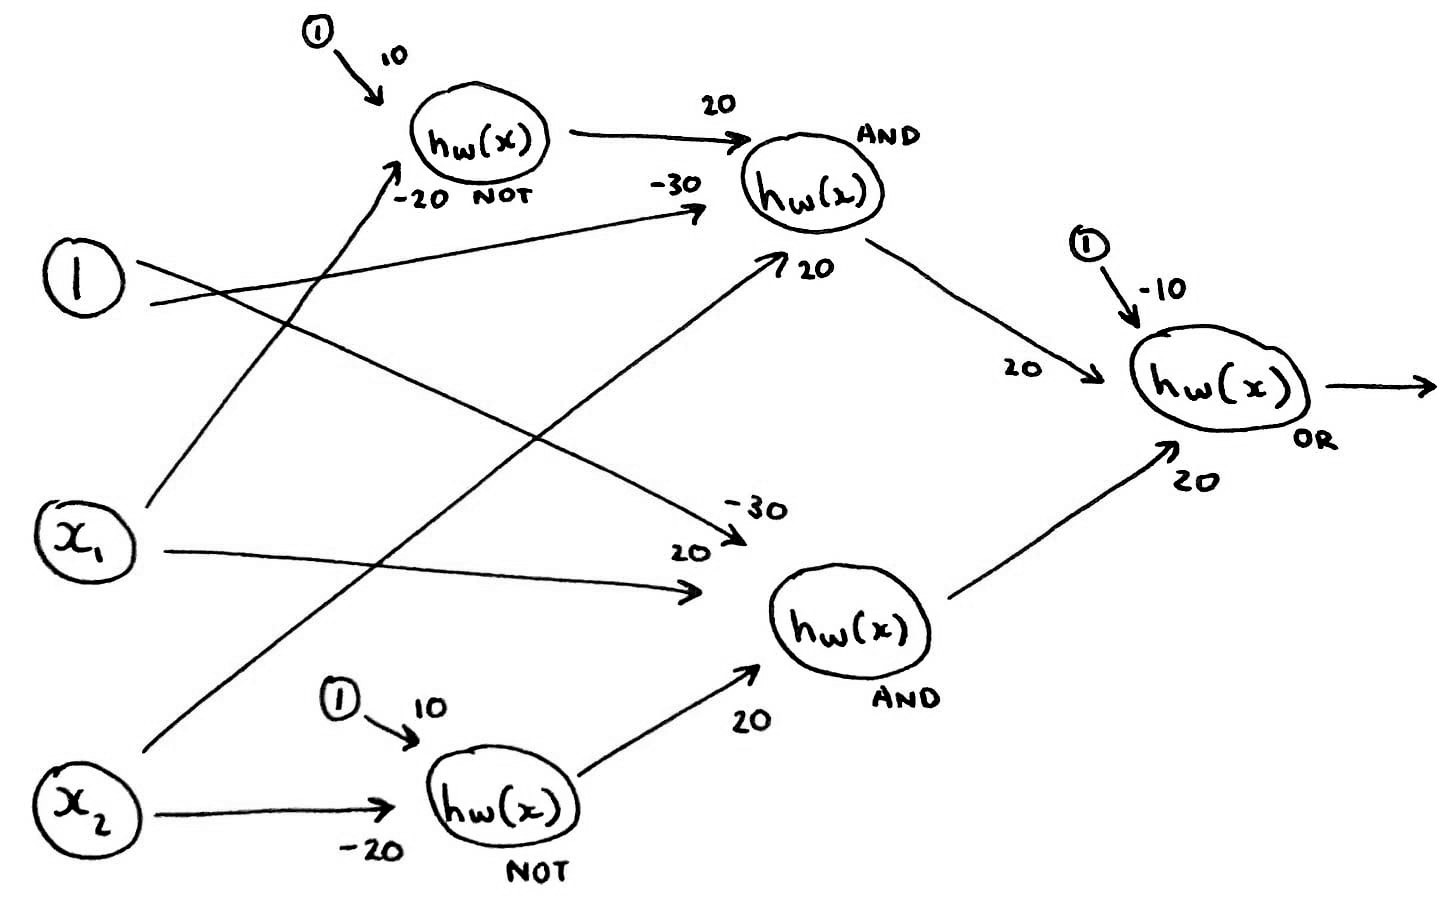
\includegraphics[scale=.4]{g3.jpeg}
\centering
\end{figure}

\begin{table}[ht]
\centering
\def\arraystretch{2}
\Large
\centering
\begin{tabular}{| p{1cm} | p{1cm} | p{1cm} | p{1cm} |}
\hline
\mathversion{bold}$x_1$ & \mathversion{bold}$x_2$ & \mathversion{bold}$z$  & \mathversion{bold}$g(z)$ \\ \hline
0  & 0  & -10 & 0  \\
0  & 1  & 20  & 1  \\
1  & 0  & 20  & 1  \\
1  & 1  & -10 & 0 \\ \hline
\end{tabular}
\end{table}

\newpage

\section*{solution1.java}
\inputminted[frame=single,framesep=10pt,mathescape=true,escapeinside=||]{java}{solution1.java}

\newpage

\section*{solution2.java}
\inputminted[frame=single,framesep=10pt,mathescape=true,escapeinside=||]{java}{solution2.java}
\end{document}